\documentclass[xcolor={usenames,dvipsnames,svgnames,table}]{beamer}
\usepackage{lmodern}

\mode<presentation> {
%\usetheme{default}
%\usetheme{AnnArbor}
%\usetheme{Antibes}
%\usetheme{Bergen}
%\usetheme{Berkeley}
%\usetheme{Berlin}
%\usetheme{Boadilla}
%\usetheme{CambridgeUS}
%\usetheme{Copenhagen}
%\usetheme{Darmstadt}
%\usetheme{Dresden}
%\usetheme{Frankfurt}
%\usetheme{Goettingen}
%\usetheme{Hannover}
%\usetheme{Ilmenau}
%\usetheme{JuanLesPins}
%\usetheme{Luebeck}
\usetheme{Madrid}
%\usetheme{Malmoe}
%\usetheme{Marburg}
%\usetheme{Montpellier}
%\usetheme{PaloAlto}
%\usetheme{Pittsburgh}
%\usetheme{Rochester}
%\usetheme{Singapore}
%\usetheme{Szeged}
%\usetheme{Warsaw}

%\usecolortheme{albatross}
%\usecolortheme{beaver}
%\usecolortheme{beetle}
%\usecolortheme{crane}
%\usecolortheme{dolphin}
%\usecolortheme{dove}
%\usecolortheme{fly}
%\usecolortheme{lily}
%\usecolortheme{orchid}
%\usecolortheme{rose}
%\usecolortheme{seagull}
%\usecolortheme{seahorse}
%\usecolortheme{whale}
%\usecolortheme{wolverine}

%\setbeamertemplate{footline} % To remove the footer line in all slides uncomment this line
%\setbeamertemplate{footline}[page number] % To replace the footer line in all slides with a simple slide count uncomment this line

\setbeamertemplate{navigation symbols}{} % To remove the navigation symbols from the bottom of all slides uncomment this line
}

\usepackage{appendixnumberbeamer} % Allows including images

\usepackage{graphicx} % Allows including images
\usepackage{booktabs} % Allows the use of \toprule, \midrule and \bottomrule in tables
\usepackage{mathtools}

\usepackage{listings}
\usepackage{courier}        % courier font
\lstset{
  basicstyle=\ttfamily
, commentstyle=\color{Green}
, keywordstyle=\bfseries\color{RoyalBlue}
, showspaces=false
, showstringspaces=false
, breaklines=true
, framextopmargin=50pt
, columns=fullflexible,keepspaces
%, frame=bottomline
      }
\setlength{\abovecaptionskip}{0pt plus 0pt minus 2pt}
\setbeamertemplate{caption}{\raggedright\insertcaption\par}

\usepackage{amsmath}
\DeclareMathOperator*{\argmin}{arg\,min}
\DeclareMathOperator*{\argmax}{arg\,max}

%----------------------------------------------------------------------------------------
%	TITLE PAGE
%----------------------------------------------------------------------------------------

\title[Compiling OCaml to C]{Compiling OCaml to C, and observing values with \lstinline{liballocs}} % The short title appears at the bottom of every slide, the full title is only on the title page

\author{Cheng Sun} % Your name
\institute[]{
CST Part II Project
}
\date{14th February 2017}

\begin{document}

\begin{frame}
\titlepage % Print the title page as the first slide
\end{frame}

%----------------------------------------------------------------------------------------
%	PRESENTATION SLIDES
%----------------------------------------------------------------------------------------

%----------------------------------------------------------------------------------------

\begin{frame}[fragile]
\frametitle{What's the problem?}

\begin{lstlisting}[language=ML,morekeywords={function}]

(* rev : 'a list -> 'a list *)
let rev xs =
    let rec loop accum = function
        | [] -> accum
        | x::xs -> loop (x::accum) xs
    in
    loop [] xs


let _ = rev [1;2;3]
\end{lstlisting}

\end{frame}

%----------------------------------------------------------------------------------------

\begin{frame}[fragile]
  \frametitle{\lstinline{ocamldebug}}

  \begin{lstlisting}[escapeinside={(*}{*)}]
(ocd) (*\aftergroup\bfseries*)break @ Test 5(*\aftergroup\mdseries*)
Loading program... done.
Breakpoint 1 at 6188: file test.ml, line 3, characters 18-94
(ocd) (*\aftergroup\bfseries*)run(*\aftergroup\mdseries*)
Time: 14 - pc: 6220 - module Test
Breakpoint: 1
5         | x::xs -> <|b|>loop (x::accum) xs
(ocd) (*\aftergroup\bfseries*)print x(*\aftergroup\mdseries*)
x: 'a = <poly>
  \end{lstlisting}

\end{frame}

%----------------------------------------------------------------------------------------

\begin{frame}[fragile]
  \frametitle{Using \lstinline{gdb} to debug OCaml programs}

  \begin{lstlisting}[escapeinside={(*}{*)}]

(gdb) (*\aftergroup\bfseries*)break test.c:20(*\aftergroup\mdseries*)
Breakpoint 1 at 0x40070d: file ./test.c, line 20.
(gdb) (*\aftergroup\bfseries*)run(*\aftergroup\mdseries*)
Starting program: /home/debian/ocaml/main

Breakpoint 1, loop_1201 (accum_1202=0x0, param_1244=0x601030) at ./test.c:20
20      intptr_t* x_1203 = param_1244[0];
(gdb) (*\aftergroup\bfseries*)next(*\aftergroup\mdseries*)
21      intptr_t* __makeblock_1255 = malloc(sizeof(intptr_t)*2);
(gdb) (*\aftergroup\bfseries*)call ocaml_liballocs_show(x_1203)(*\aftergroup\mdseries*)
1
\end{lstlisting}

\end{frame}


%----------------------------------------------------------------------------------------

\begin{frame}
  \frametitle{My approach}


\begin{figure}[H]
  \begin{overprint}
    \onslide<1>
  \centering
  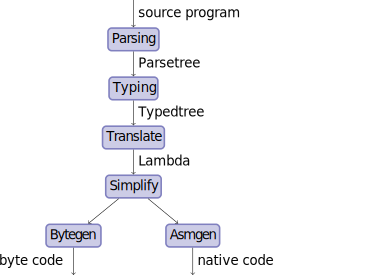
\includegraphics[height=16em]{presentation_2alt}

  \caption{\tiny\textit{(adapted from Fischbach 2011)}}

    \onslide<2>
  \centering
  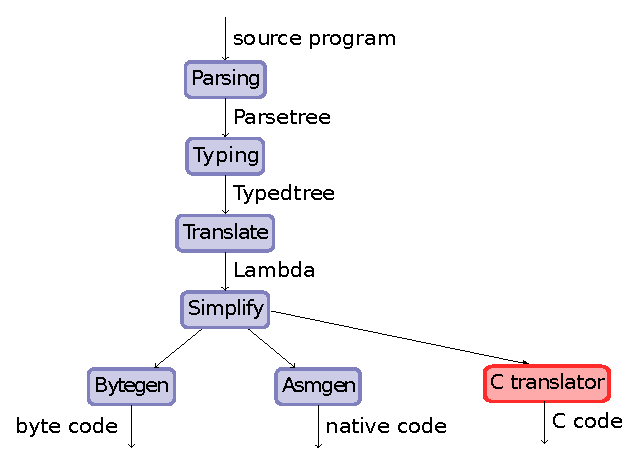
\includegraphics[height=16em]{presentation_2}

  \caption{\tiny\textit{(adapted from Fischbach 2011)}}

    \onslide<3>
  \centering
  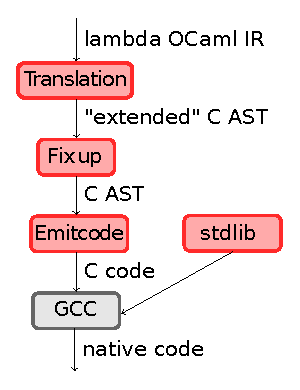
\includegraphics[height=16em]{presentation_3}
\end{overprint}
\end{figure}

\end{frame}


%----------------------------------------------------------------------------------------

\begin{frame}[fragile]
\frametitle{What's done so far?}

Enough to get some self-contained OCaml programs running.

\begin{enumerate}
  \item Basic types
  \item Tuples, lists, records, references
  \item Polymorphic functions
  \item Cross-module interfacing
  \item Prototype standard library (\lstinline{List}, \lstinline{Printf})
  \item Test suite of self-contained OCaml programs
\end{enumerate}

\end{frame}


%----------------------------------------------------------------------------------------

\begin{frame}[fragile]
\frametitle{What's next?}

\begin{enumerate}
  \item Closures
  \item Better types representation with \lstinline{liballocs}
  \item Better debugging experience
  \item Evaluation
\end{enumerate}

\end{frame}



%----------------------------------------------------------------------------------------

\appendix

%----------------------------------------------------------------------------------------

\begin{frame}[fragile]
  \frametitle{A snippet of C output}

  \begin{lstlisting}[language=C,basicstyle=\ttfamily\scriptsize,morekeywords={intptr_t}]
intptr_t* loop_1201(intptr_t* accum_1202, intptr_t* param_1244){
intptr_t* __deinlined_1256;
if (param_1244) {
intptr_t* xs_1204 = param_1244[1];
intptr_t* x_1203 = param_1244[0];
intptr_t* __makeblock_1255 = malloc(sizeof(intptr_t)*2);
__makeblock_1255[0] = x_1203;
__makeblock_1255[1] = accum_1202;
__deinlined_1256 = ((intptr_t*(*)(intptr_t*,intptr_t*))loop_1201)(__makeblock_1255, xs_1204);
} else {
__deinlined_1256 = accum_1202;
}
return __deinlined_1256;
}

intptr_t* rev_1199(intptr_t* xs_1200){
loop_1201;
return ((intptr_t*(*)(intptr_t*,intptr_t*))loop_1201)(((void*)0), xs_1200);
}

\end{lstlisting}

\end{frame}

%%------------------------------------------------
%\section{The game of go}
%%------------------------------------------------
%
%%----------------------------------------------------------------------------------------
%
%\begin{frame}
%\frametitle{Introduction to go}
%Go is an abstract board game with deceptively simple rules.
%
%\begin{itemize}
%  \item Black and white take turns placing stones, or passing
%    % once a stone is placed, it cannot be moved.
%  \item Orthogonally adjacent points are liberties
%  \item A stone with no liberties is captured
%
%    \centerline{\includegraphics[height=8em]{Golibs}\qquad \includegraphics[height=8em]{Go_capturing}}
%  \item Groups share liberties, hence must be captured all at once
%  \item The game ends when both players consecutively pass
%  \item The player controlling the most ``territory'' at the end wins
%\end{itemize}
%
%% disclaimer
%\end{frame}
%
%%----------------------------------------------------------------------------------------
%
%\begin{frame}
%  \frametitle{Example game}
%
%  The ``ear-reddening game'': Honinbo Shusaku (black) and Inoue Genan Inseki (white), 1846.
%
%  \only<1>{
%    \centerline{\includegraphics[height=15em]{ear-red}}
%  }
%  \only<2>{
%    \centerline{\includegraphics[height=15em]{ear-red2}}
%  }
%
%\end{frame}
%
%\begin{frame}
%  \frametitle{Game-playing AIs}
%
%  In the game tree, each node is a \textit{position}, and each edge is an \textit{action}.
%
%    \centerline{\includegraphics[height=8em]{search_tree}}
%
%  \textbf{Evaluate}:
%  \begin{itemize}
%    \item Assign a \textit{value} to a position
%    \item Contains many domain-specific heuristics
%  \end{itemize}
%
%  \textbf{Search}:
%  \begin{itemize}
%    \item Based on the \textit{minimax} principle
%    \item Want ways to prune useless branches to reduce the \textbf{branching factor}
%    \item Traditionally an $\alpha\beta$ search
%  \end{itemize}
%
%  % Brief introduction to concepts, terminology
%  % Zero-sum game
%\end{frame}
%
%%----------------------------------------------------------------------------------------
%
%\begin{frame}
%  \frametitle{Recent advancements in chess}
%
%  In computer chess, there have been significant advancements in \textbf{search}:
%
%\begin{columns}[c]
%
%\column{.45\textwidth} % Left column and width
%\begin{itemize}
%  \item Principal variation search
%  \item Quiescence search
%  \item Check extensions
%  \item Capture extensions
%  \item Late move reductions
%  \item Futility pruning and razoring
%  \item Static exchange evaluation
%\end{itemize}
%
%\column{.5\textwidth} % Right column and width
%
%
%\begin{figure}[H]
%  \centering
%  \includegraphics[width=.5\textwidth]{chess}
%  \caption{\tiny\textit{(White to move)}}
%\end{figure}
%
%\end{columns}
%
%\bigskip
%
%  These techniques result in an effective branching factor of \textbf{less than 2}.
%\end{frame}
%
%%----------------------------------------------------------------------------------------
%
%\begin{frame}
%\frametitle{Traditional search in go}
%
%Traditional $\alpha\beta$ search doesn't work well for go. Why?
%
%\begin{itemize}
%  \item Hard to evaluate
%\begin{itemize}
%  \item Can't ``count pieces'' for a rough estimate
%  \item Determining if a group is alive or dead is NP-hard (Cr\^{a}\c{s}maru, 1999)
%\end{itemize}
%  \item Additive nature (position gets more complex as time goes on)
%  \item Almost every move is legal, and a large number of moves have some value
%  \item Large ($19\times19$) board
%\end{itemize}
%\end{frame}
%
%%----------------------------------------------------------------------------------------
%
%\begin{frame}
%\frametitle{History of go engines}
%
%\centerline{\includegraphics[scale=1.2]{rankings}}
%
%\begin{figure}[H]
%  \centering
%\fbox{
%  \includegraphics[scale=.6]{engineprogression}
%}
%  \caption{\tiny\textit{(Ratings taken from the KGS Go server)}}
%\end{figure}
%
%\vspace*{-2em}
%
% % 1990: 15 kyu
% % 9x9 professional level
% % 19x19 very strong amateur level
%\end{frame}
%
%
%%----------------------------------------------------------------------------------------
%
%\subsection{Flat Monte Carlo algorithm}
%
%\begin{frame}
%\frametitle{Monte Carlo: philosophy}
%
%\begin{itemize}
%  \item If a good \textbf{evaluation} is too hard, try \textbf{simulation} instead.
%  \item Play many random games starting from a given position
%\end{itemize}
%
%\vspace*{-1em}
%\begin{figure}[H]
%  \centering
%  \includegraphics[scale=.65]{mcbasic}
%  \caption{\tiny\textit{(Coulom, 2008)}}
%\end{figure}
%\end{frame}
%
%%----------------------------------------------------------------------------------------
%
%\begin{frame}
%\frametitle{Flat Monte Carlo algorithm}
%
%The Flat Monte Carlo algorithm uses simulation to choose the best \textit{action}:
%
%\begin{figure}[H]
%  \centering
%  \includegraphics[scale=.6]{mcexample}
%  \caption{\tiny\textit{(Coulom, 2008)}}
%\end{figure}
%
%\vspace{-2em}
%
%  \begin{itemize}
%    \item \textbf{Selection}: Pick a child uniformly at random
%    \item \textbf{Playout}: Simulate until the end of the game, by playing random moves
%    \item \textbf{Back-propagation}: Update win statistics for the action
%  \end{itemize}
%
%  Repeat until we have exceeded our \textit{computational budget}
%
%\end{frame}
%
%%----------------------------------------------------------------------------------------
%
%\begin{frame}
%\frametitle{Flat Monte Carlo algorithm}
%
%  Advantages:
%  \begin{itemize}
%    \item Anytime: best estimate always available
%    \item Parallelisable: embarrassingly so
%  \end{itemize}
%
%  Disadvantages:
%  \begin{itemize}
%    \item Symmetric: all actions treated uniformly
%    \item Not consistent: does not necessarily converge to optimum
%  \end{itemize}
%\end{frame}
%
%%----------------------------------------------------------------------------------------
%
%\begin{frame}
%  \frametitle{The multi-armed bandit problem}
%
%  We want a smarter \textbf{selection}: instead of picking uniformly from $K$ children\ldots
%
%\begin{figure}[H]
%  \centering
%  \includegraphics[scale=.2]{bandits}
%  \includegraphics[scale=.2]{bandits}
%  \includegraphics[scale=.2]{bandits}
%  \includegraphics[scale=.2]{bandits}
%\end{figure}
%\vspace*{-1em}
%  \begin{itemize}
%    \item Treat the problem like playing $K$ slot machines (``arms''), each with unknown rewards.
%
%    \item Each arm $k$ gives 0 or 1 reward, with mean $\mu_{k}$.
%
%    \item The arm $k^*$ has the highest expected reward $\mu_{k^*}$.
%
%    \item We find out more about the arms the more we play
%
%    \item Objective: after playing arms $k(1)$, $k(2)$, \ldots, $k(n)$, minimise the \textbf{cumulative regret}
%      \[\sum_{t=1}^{n} (\mu_{k^*} - \mu_{k(t)})\]
%  \end{itemize}
%\end{frame}
%
%%----------------------------------------------------------------------------------------
%
%\begin{frame}
%  \frametitle{MAB: greedy strategy}
%
%\bigskip
%  Write the \textit{empirical mean} of arm $k$ at time $t$ as $\hat\mu_{k,t}$.
%
%  \begin{block}{Greedy strategy}
%    \textit{``Pick the child with the best observed value so far.''}
%    \bigskip
%
%    At time $t$, pick
%    \[k(t) = \argmax_{i} \hat\mu_{i,t}\]
%  \end{block}
%
%  Problem?
%
%  \begin{overprint}
%    \onslide<1>
%
%    \begin{columns}
%\column{.3\textwidth} % Left column and width
%\column{.1\textwidth} % Left column and width
%\begin{figure}[H]
%  \centering
%  \includegraphics[scale=.2]{bandits}
%  \caption{A: $1/3$}
%\end{figure}
%\column{.1\textwidth} % Left column and width
%\begin{figure}[H]
%  \centering
%  \includegraphics[scale=.2]{bandits}
%  \caption{B: $2/3$}
%\end{figure}
%\column{.3\textwidth} % Left column and width
%\end{columns}
%
%\onslide<2>
%  \begin{itemize}
%    \item We want to minimise regret by \textbf{exploiting} the best arm
%    \item Greedy strategy fails because we don't \textbf{explore} other options
%  \end{itemize}
%
%  %The key problem with the algorithm above is that we’re too certain
%  %of our estimates. When we have seen a single reward of 0 we
%  %shouldn’t conclude the average reward is 0, but rather than it lies
%  %within some
%  %confidence interval.
%
%\end{overprint}
%
%\end{frame}
%%----------------------------------------------------------------------------------------
%
%\begin{frame}
%  \frametitle{Upper-Confidence Bound}
%
%  We should explore arms which we don't know much about, by
%  constructing \textit{confidence intervals} for $\mu_k$.
%
%  \begin{block}{UCB1 strategy (Auer et al, 2002)}
%    \textit{Optimism in the face of uncertainty: ``Choose the child with the highest optimistic value estimate.''}
%
%    \bigskip
%
%    Define the upper-confidence bound of arm $k$ at time $t$ as:
%    \[B_{k,t} = \hat\mu_{k,t} + \sqrt{\frac{2\log t}{T_k(t)}}\]
%    where $T_k(t)$ is the number of times arm $k$ has been played up to time $t$.
%
%    Pick:
%    \[k(t) = \argmax_{i} B_{i,t}\]
%  \end{block}
%
%  % The first term is the exploitation term, the second the exploration term
%\end{frame}
%
%\begin{frame}
%  \frametitle{UCB: demo}
%
%  \centerline{This slide intentionally left blank}
%\end{frame}
%
%\begin{frame}
%  \frametitle{UCB: optimality}
%
%  We will prove that following the UCB1 strategy, cumulative regret grows as $O(\log t)$.
%
%  \bigskip
%
%  Lai and Robbins (1985) proved that no multi-armed bandit strategy has better than logarithmic growth of regret.
%
%\end{frame}
%
%%----------------------------------------------------------------------------------------
%
%\begin{frame}<1-3>[label=ucb-optimal]
%\frametitle{UCB: proof of logarithmic growth of cumulative regret}
%
%\only<1> {
%Say that we choose a suboptimal arm $k$ at time $t$. Then
%\begin{align*}
%  B_{k,t} &\ge B_{k^*,t} \\
%  \implies \quad \hat\mu_{k,t} + \sqrt{\frac{2\log t}{T_{k}(t)}} &\ge \hat\mu_{k^*,t} + \sqrt{\frac{2\log t}{T_{k^*}(t)}} \phantom{\implies\quad}
%\end{align*}
%
%With high probability, both arms' distribution means lie in our confidence intervals. In particular:
%}
%
%\begin{columns}[c]
%\column{.4\textwidth} % Left column and width
%\begin{equation}
%  \label{eq:1}
%  \mu_{k} \stackrel{\mathclap{\text{\tiny whp}}}{\ge} \hat\mu_{k,t} - \sqrt{\frac{2\log t}{T_{k}(t)}}
%\end{equation}
%
%\column{.4\textwidth} % Left column and width
%\begin{equation}
%  \label{eq:2}
%  \mu_{k^*} \stackrel{\mathclap{\text{\tiny whp}}}{\le} \hat\mu_{k^*,t} + \sqrt{\frac{2\log t}{T_{k^*}(t)}}
%\end{equation}
%\end{columns}
%
%\bigskip
%
%\only<2-> {
%
%  \begin{overprint}
%    \onslide<2>
%
%If conditions \eqref{eq:1} and \eqref{eq:2} hold, then
%\begin{alignat*}{2}
%  &&\hat\mu_{k,t} + \sqrt{\frac{2\log t}{T_{k}(t)}} &\ge \hat\mu_{k^*,t} + \sqrt{\frac{2\log t}{T_{k^*}(t)}} \\
%  \implies &&\mu_{k^*} - \mu_{k} &\le 2\sqrt{\frac{2\log t}{T_{k}(t)}} \\
%  \implies &&T_{k}(t) &\le \frac{8\log t}{(\mu_{k^*} - \mu_{k})^2}
%\end{alignat*}
%
%\onslide<3>
%  In this case, we can bound the cumulative regret:
%\begin{align*}
%  \sum_{t=1}^{n} (\mu_{k^*} - \mu_{k(t)}) &= \sum_{k=1}^{K} (\mu_{k^*} - \mu_{k}) T_k(n) \\
%  &\le \log n \sum_{\substack{1\le k\le K \\ k\ne k^*}} \frac{8}{\mu_{k^*} - \mu_{k}}
%\end{align*}
%
%Complete proof given by Auer et al (2002) bounds the probability of conditions \eqref{eq:1} and \eqref{eq:2} failing using the \textit{Chernoff-Hoeffding bound}.
%
%The expected regret remains bounded by $O(\log n)$.
%
%  \onslide<4>
%We may end up playing arm $k$ too much, if either condition fails at any time $t$ ($1 \le t \le n$). Hence an unconditional upper bound is
%\[
%  T_k(n) \le \left\lceil\frac{8\log n}{(\mu_{k^*} - \mu_{k})^2}\right\rceil + \sum_{t=1}^{n}\mathbf{I}[\mbox{Either condition fails at time $t$}]
%\]
%
%\onslide<5>
%By the Chernoff-Hoeffding bound,
%\begin{align*}
%  \mathbb{P}(\mbox{Condition \eqref{eq:1} fails at time $t$}) &\le t^{-2} \\
%  \mathbb{P}(\mbox{Condition \eqref{eq:2} fails at time $t$}) &\le t^{-2}
%\end{align*}
%
%Then by taking expectations we have
%\begin{align*}
%  \mathbb{E}[T_k(n)] &\le \left\lceil\frac{8\log n}{(\mu_{k^*} - \mu_{k})^2}\right\rceil + \sum_{t=1}^{n}2t'^{-2} \\
%  &\le \frac{8\log n}{(\mu_{k^*} - \mu_{k})^2} + 1 + \frac{\pi^2}{3} && \mbox{(Basel problem)}
%\end{align*}
%
%\onslide<6>
%  The expected cumulative regret is still bounded:
%
%\begin{align*}
%  \mathbb{E}\left[\sum_{t=1}^{n} (\mu_{k^*} - \mu_{k(t)})\right] &= \sum_{k=1}^{K} (\mu_{k^*} - \mu_{k(t)}) \mathbb{E}[T_k(n)] \\
%  &\le \log t \sum_{\substack{1\le k\le K \\ k\ne k^*}} \frac{8}{\mu_{k^*} - \mu_{k}} + K\left(1 + \frac{\pi^2}{3}\right)
%\end{align*}
%
%\end{overprint}
%}
%
%\end{frame}
%
%%----------------------------------------------------------------------------------------
%
%\begin{frame}
%  \frametitle{Monte Carlo simulation inconsistency}
%
%  \begin{itemize}
%      \item
%  No matter what \textbf{selection} strategy we choose, the \textbf{playout policy} is the weak link in the Flat Monte Carlo algorithm.
%
%      \item
%  Flat Monte Carlo easily falls prey to tactical situations:
%  \end{itemize}
%
%\vspace*{-1em}
%
%\begin{figure}[H]
%  \centering
%  \includegraphics[scale=.3]{mcfail}
%\end{figure}
%
%\vspace*{-1em}
%
%  \begin{itemize}
%      \item
%  Problem: there is no ``opponent model''
%      \item
%  Idea: use history of multi-armed bandit selection to incrementally build a tree
%  \end{itemize}
%\end{frame}
%
%%----------------------------------------------------------------------------------------
%
%\begin{frame}
%  \frametitle{Monte Carlo Tree Search}
%
%  Introduced by Coulom (2006) in a paper that began the go AI revolution
%
%\begin{figure}[H]
%  \centering
%  \includegraphics[width=.8\textwidth]{mcts_steps}
%  \caption{\tiny\textit{(Browne et al, 2012)}}
%\end{figure}
%
%\vspace*{-1em}
%
%  \textit{Tree policy}: The search tree is used to guide the first part of the search
%  \textit{Default policy}: MC simulation used for the rest of the game
%
%  \bigskip
%
% %\begin{enumerate}
% %  \item Selection: select child recursively until an incomplete node is reached
% %  \item Expansion: add a random new child node; use this as our root position for playout
% %  \item Playout: use Monte Carlo simulation to play the game
% %  \item Back-propagation: Update the statistics on all nodes back up to the root
% %\end{enumerate}
%
%  %Starts off choosing actions uniformly, but eventually focuses on the best actions, according to previously observed rewards.
%  % Note, selection happens in perspective of player whose action it is (minimax principle)
%\end{frame}
%
%
%\begin{frame}
%  \frametitle{Monte Carlo Tree Search}
%
%  Maintains all advantages of Monte Carlo simulation, and overcomes the biggest disadvantages.
%
%  \begin{columns}[c]
%    \column{.45\textwidth} % Left column and width
%      \begin{itemize}
%        \item Anytime
%        \item Parallelisable % not as much: parallel searches can't use info from searches happening at the same time
%        \item Asymmetric: promising branches are explored deeper
%        \item Consistent?
%      \end{itemize}
%
%    \column{.45\textwidth} % Left column and width
%    \begin{figure}[H]
%      \centering
%      \includegraphics[width=\textwidth]{asymmetry}
%      \caption{\tiny\textit{(Browne, 2012)}}
%    \end{figure}
%  \end{columns}
%\end{frame}
%
%%----------------------------------------------------------------------------------------
%
%\begin{frame}
%  \frametitle{UCT}
%
%  Upper Confidence Trees refers to MCTS with UCB1 as the selection policy.
%
%  UCT can be shown to be a consistent strategy (Kocsis and Szepesv\'ari, 2006).
%
%  Proof outline:
%  \begin{itemize}
%    \item Each node is visited infinitely often
%    \item Nodes' values can be inductively proven to tend to the value of its' optimal child(ren).
%    \item Hence root node tends towards the true value
%  \end{itemize}
%\end{frame}
%
%%----------------------------------------------------------------------------------------
%
%\begin{frame}
%  \frametitle{Refinements: AMAF and RAVE}
%
%  \textbf{All Moves As First} (AMAF) heuristic
%  \begin{itemize}
%    \item ``a good move is probably good no matter when it is played''
%    \item During back-propagation, actions also update values as if they were played from previous positions
%  \end{itemize}
%\bigskip
%\textbf{Rapid-Action Value Estimate} refinement (Gelly and Silver, 2007)
%  \begin{itemize}
%    \item Record AMAF and MC simulation values separately
%    \item Interpolate between the two to give a hybrid value
%    \item AMAF dominates at beginning, then tapers off with more simulation results
%  \end{itemize}
%
%  %Advantage:
%  %Gives bandit selection strategy something to work with at the beginning
%
%  %Disadvantage:
%  %Tactical moves may be heavily dependent on context
%
%\end{frame}
%
%%----------------------------------------------------------------------------------------
%
%\begin{frame}
%\frametitle{Current research}
%\textbf{Biasing selection with domain-specific knowledge}
%
%The bandit strategy should first select an action if it is likely to be strong, according to:
%\begin{itemize}
%  \item Opening databases
%  \item Pattern databases
%  \item Life and death heuristics
%  \item Neural networks (Maddison et al, 2015)
%\end{itemize}
%
%NB: maintaining consistency when biased is hard (Berthier et al, 2010)
%
%\bigskip
%
%\textbf{Alternative bandit strategies}
%\begin{itemize}
%  \item Optimising \textbf{simple regret} instead?
%  \item SHOT: Sequential Halving On Trees, an alternative to UCT (Cazenave, 2014)
%  \item H-MCTS: hybrid SHOT/UCT policy (Pepels et al., 2014)
%\end{itemize}
%
%\end{frame}
%
%\begin{frame}
%\frametitle{Current research}
%\textbf{Monte Carlo Tree Search}
%\begin{itemize}
%  \item Dominating computer go: can now beat professional 9-dan players with a 4-stone handicap
%  \item World champion at Hex
%  \item Can be applied to non-deterministic games, such as backgammon, poker and Ms. Pac-Man
%\end{itemize}
%
%\bigskip
%
%\textbf{Multi-armed bandit theory} is being applied to:
%\begin{itemize}
%  \item Clinical trials
%  \item Ad placement on web pages
%  \item Investment / resource allocation
%\end{itemize}
%\end{frame}
%
%%----------------------------------------------------------------------------------------
%
%\begin{frame}
%\Huge{\centerline{Questions?}}
%
%\bigskip
%\bigskip
%
%\centerline{\includegraphics[width=0.9\textwidth]{reassuring}}
%\end{frame}
%
%%----------------------------------------------------------------------------------------
%
%\appendix
%
%%----------------------------------------------------------------------------------------
%
%\begin{frame}
%\frametitle{History of go engines}
%\begin{itemize}
%  \item Prior to 2006: pattern databases, ad-hoc heuristics and $\alpha\beta$ search, e.g. in \textit{GNU Go} ($\sim 1800$ Elo)
%  \item Bouzy (2003): Monte Carlo simulations, in \textit{Indigo} ($\sim 1400$ Elo)
%  \item Coulom (2006): Monte Carlo Tree Search (MCTS), in \textit{Crazy Stone} ($\sim 1600$ Elo)
%  \item Kocsis and Szepesv\'ari (2006): Upper-Confidence Trees (UCT)
%  \item Gelly and Silver (2007): Rapid Action Value Estimate (RAVE), in \textit{MoGo} ($\sim 2300$ Elo)
%\end{itemize}
%
%\begin{block}{Elo rating}
%  A 200 Elo difference means the stronger player will win 75\% of the time.
%
%  A 700 Elo difference means the stronger player will win 99\% of the time.
%\end{block}
%
% % All modern engines now use MCTS.
%
%\end{frame}
%
%%----------------------------------------------------------------------------------------
%
%\begin{frame}
%  \frametitle{MAB: $\epsilon$-greedy strategy}
%
%  Choose a parameter $\epsilon$ such that $0 \le \epsilon \le 1$.
%
%  \begin{block}{$\epsilon$-greedy strategy}
%    \textit{``Pick the child with the best observed value most of the time, but sometimes try one of the others too.''}
%    \bigskip
%
%    With probability $\epsilon$, pick an arm uniformly at random.
%
%    Otherwise, pick:
%    \[k(t) = \argmax_{i} \hat\mu_{i,t}\]
%  \end{block}
%
%\end{frame}
%
%%----------------------------------------------------------------------------------------
%
%\begin{frame}
%  \frametitle{$\epsilon$-greedy selection policy for MCTS}
%
%  \begin{itemize}
%    \item We can apply the $\epsilon$-greedy selection policy for MCTS\ldots
%    \item \ldots but it's not consistent!
%  \end{itemize}
%
%\begin{figure}[H]
%  \centering
%  \includegraphics[scale=0.7]{egreedy}
%  \caption{\tiny\textit{(Berthier et al, 2009)}}
%\end{figure}
%\end{frame}
%
%\againframe<4>{ucb-optimal}
%
%\begin{frame}{Chernoff-Hoeffding bound}
%  Let $X_1\dots X_n$ be random variables with common range $[0,1]$, such that $\mathbb{E}[X_t | X_1, \dots, X_{t-1}] = \mu$.
%
%  \bigskip
%
%Let $S_n = \sum_{i=1}^n X_i$.
%
%  \bigskip
%
%Then for all $a\ge0$:
%
%\begin{align*}
%  \mathbb{P}(S_n\ge n\mu + a) &\le e^{-2a^2/n} \\
%  \mathbb{P}(S_n\le n\mu - a) &\le e^{-2a^2/n}
%  \end{align*}
%\end{frame}
%
%\againframe<5->{ucb-optimal}

\end{document}

% vim: ts=2 sts=2 sw=2 et
